\documentclass[conference]{IEEEtran}
\usepackage{amsmath,amssymb}
\usepackage{graphicx}
\usepackage{cite}
\usepackage{textcomp}
\usepackage{xcolor}
\usepackage{booktabs}
\usepackage[colorlinks=true, linkcolor=blue, citecolor=blue, urlcolor=blue]{hyperref}

% Strict float placement controls for 6-page conference formatting
\setcounter{topnumber}{2}
\setcounter{bottomnumber}{2}
\setcounter{totalnumber}{4}
\setcounter{dbltopnumber}{2}
\renewcommand{\dbltopfraction}{0.90}
\renewcommand{\topfraction}{0.90}
\renewcommand{\bottomfraction}{0.80}
\renewcommand{\textfraction}{0.10}
\renewcommand{\floatpagefraction}{0.75}
\setlength{\textfloatsep}{6pt plus 1pt minus 1pt}
\setlength{\dbltextfloatsep}{6pt plus 1pt minus 1pt}
\setlength{\floatsep}{4pt plus 1pt minus 1pt}
\setlength{\dblfloatsep}{4pt plus 1pt minus 1pt}
\setlength{\intextsep}{4pt plus 1pt minus 1pt}

\begin{document}

\title{AI-ML Based Intelligent Dead Reckoning and 3D Map-Matching System for Seamless Navigation}

\author{
\IEEEauthorblockN{1\textsuperscript{st} Shreya Kesarwani}
\IEEEauthorblockA{\small Computer Science and Engineering\\
United College of Engineering \& Research\\
Prayagraj, India\\
kesarwanishreya2005@gmail.com}
\and
\IEEEauthorblockN{2\textsuperscript{nd} Akash Mishra}
\IEEEauthorblockA{\small Computer Science and Engineering\\
United College of Engineering \& Research\\
Prayagraj, India\\
akashmishra1910@gmail.com}
\and
\IEEEauthorblockN{3\textsuperscript{rd} Suchitra}
\IEEEauthorblockA{\small Computer Science and Engineering\\
United College of Engineering \& Research\\
Prayagraj, India\\
mesuchitradutta@gmail.com}
}

\maketitle

\begin{abstract}
Smartphone navigation systems are the primary positioning consoles for vehicular transit across dense corridors where Global Navigation Satellite System (GNSS) reception regularly degrades in tunnels, underpasses, urban canyons, and multi-tier flyovers. However, consumer smartphone MEMS inertial measurement units (IMUs) suffer from stochastic bias drift and severe road vibrations, causing unconstrained double integration to accumulate hundreds of meters of positional error within seconds. In this work, we propose an edge-deployable Intelligent Dead Reckoning (IDR) and 3D map-matching framework that operates framework-free on commodity smartphones without vehicle OBD-II telemetry. Following offline training in Python, the GBDT forward-velocity regressor and shock filter are compiled into native C++ decision lookup tables that execute with zero external deep learning runtime dependencies. The system tightly couples dynamic gravity leveling, an in-vehicle cradle alignment watchdog, a 15-state Error-State Kalman Filter (ESKF) with data-driven Non-Holonomic Constraints (NHC) and Zero-Velocity Updates (ZUPT), and an elevation-aware 3D topological map-matcher. Evaluated on a high-fidelity trajectory emulation platform adhering to the IO-VNBD benchmark schema \cite{onyekpe2021} alongside an empirical on-road driving trial on real smartphone hardware with dual-frequency RTK-GNSS ground truth, all baseline models and proposed configurations are directly implemented and evaluated on identical tracks. On continuous cruising corridors, the proposed 15-state ESKF bounds drift to $2.01 \pm 0.18\%$ at 60\,s and $2.88 \pm 0.24\%$ at 120\,s, substantially outperforming directly re-run strapdown double integration (61.5\% at 60\,s) and standalone AI velocity estimation (27.9\% at 60\,s). Under urban stop-and-go outages with traffic halts, ZUPT actively reduces drift from 4.61\% to 2.58\% (a 44.0\% relative error reduction). Furthermore, the 3D map-matcher bounds full-system endpoint drift to 1.72\% (60\,s) and 2.80\% (120\,s) with 99.7\%--100\% flyover disambiguation accuracy at an end-to-end single-epoch cycle latency of $0.20 \pm 0.02$\,ms on mobile hardware.
\end{abstract}

\begin{IEEEkeywords}
dead reckoning, sensor fusion, GNSS-denied navigation, error-state Kalman filter, map matching, machine learning, non-holonomic constraints.
\end{IEEEkeywords}

\section{Introduction}

\subsection{Background}
Vehicle logistics, ride-hailing fleets, and emergency-response services rely heavily on smartphone navigation applications utilizing constellations such as GPS, Galileo, GLONASS, and NavIC. In emerging transport ecosystems such as India, smartphones mounted on dashboards or windshield cradles serve as the primary computing and navigation console across commercial vehicles. These fleets lack factory-installed, wheel-odometry-coupled Inertial Navigation Systems (INS). Consequently, when vehicles enter GNSS-denied environments---such as urban canyons, vehicular tunnels, underpasses, and multi-level flyovers---satellite signals suffer severe attenuation, multipath reflections, or complete outage, causing conventional turn-by-turn navigation to diverge rapidly. In automotive navigation, a cumulative positional drift below 10\% of distance traveled constitutes the recognized operational benchmark tolerance, ensuring that navigation software does not trigger false off-route recalculations before satellite re-acquisition.

Inertial dead reckoning (DR) provides self-contained positioning that is immune to satellite obscuration, jamming, and spoofing \cite{brossard2020, lawal2024}. However, consumer smartphone MEMS sensors exhibit substantial stochastic bias drift, thermo-mechanical noise, and scale-factor errors. Double integrating uncorrected accelerations causes positional error to accumulate quadratically over time. Furthermore, a smartphone mounted inside a vehicle experiences large extraneous accelerations induced by engine idle vibrations, abrupt braking, and road surface irregularities (potholes and speed bumps) that do not reflect true center-of-mass vehicular displacement.

\subsection{Problem Statement}
Two practical challenges prevent classical inertial dead reckoning from operating reliably on commodity smartphones:
\begin{enumerate}
\item \textbf{Absence of Direct Speedometer Telemetry}: Without access to the vehicle OBD-II diagnostic port or CAN bus, forward wheel speed cannot be directly observed. Longitudinal velocity must be estimated purely from noisy, gravitationally coupled accelerometer and gyroscope streams \cite{brossard2020, qian2025}.
\item \textbf{Arbitrary Orientation, Cradle Slip, and Road Shocks}: Smartphones are placed arbitrarily in commercial cradles without mechanical alignment to the vehicle chassis. Road vibrations (15--30\,Hz engine idle) and severe pothole impulses ($\le 3.2g$) rapidly corrupt double integration. Furthermore, sharp cornering can cause the phone to slip or tilt within its cradle, destroying coordinate transformations and attitude estimation unless detected and re-calibrated in real time \cite{matos2025}.
\end{enumerate}

\subsection{Aim and Contributions}
This paper presents a complete, edge-deployable framework (Fig.~\ref{fig:overall_arch}) that maintains accurate, drift-bounded 3D vehicle positioning during extended GNSS outages without OBD-II telemetry. Following offline training in Python, the GBDT forward-velocity regressor and shock filter are compiled into native C++ decision lookup tables that execute framework-free on device with zero external deep learning runtime dependencies (e.g., zero dependencies on PyTorch Mobile, TensorFlow Lite, or ONNX Runtime). The primary contributions are:
\begin{itemize}
\item An end-to-end Intelligent Dead Reckoning (IDR) architecture integrating dynamic gravity leveling, longitudinal PCA alignment with a slip watchdog, a native C++ regularized GBDT forward-velocity and shock filter \cite{friedman2001}, a 15-state ESKF with Non-Holonomic Constraints (NHC) \cite{dissanayake2001} and ZUPT \cite{foxlin2005}, and a 3D elevation-aware HMM map-matcher \cite{newson2009}.
\item A unified mathematical formulation linking coordinate transformations, machine learning pseudo-measurements, error-state propagation \cite{sola2017}, and probabilistic 3D Viterbi map matching.
\item Systematic empirical validation across both high-fidelity trajectory emulation adhering to the IO-VNBD benchmark schema \cite{onyekpe2021} and an empirical on-road smartphone driving trial with RTK-GNSS ground truth. Baseline methods \cite{dissanayake2001, brossard2020} are directly implemented and re-run on identical corridors, demonstrating ESKF continuous drift bounded to $2.01 \pm 0.18\%$ (60\,s) and $2.88 \pm 0.24\%$ (120\,s) on continuous cruising, an active $44.0\%$ drift reduction from ZUPT during urban stop-and-go halts, full-system endpoint drift bounded to $\le 2.80\%$, $99.7\%$--$100\%$ flyover disambiguation, and a single-step latency of $0.20 \pm 0.02$\,ms on mobile hardware.
\end{itemize}

\section{Related Work}

Vehicular dead reckoning and localization have evolved across classical strapdown inertial navigation \cite{dissanayake2001, foxlin2005}, machine learning state estimators \cite{brossard2020, lawal2024, qian2025, mamun2026}, and road-network map matching \cite{newson2009, javed2024, sundar2026}. Classical strapdown INS double-integrates triaxial specific force and angular rates, but low-cost MEMS sensor biases trigger rapid quadratic divergence unless aided by kinematic constraints such as Non-Holonomic Constraints (NHC) \cite{dissanayake2001} and Zero-Velocity Updates (ZUPT) \cite{foxlin2005}. However, classical methods require direct wheel odometry or strict stationary conditions to bound error growth.

Recent deep learning approaches estimate forward velocity or correct inertial errors using neural sequence models \cite{brossard2020, lawal2024, mamun2026}. Qian et al. \cite{qian2025} regressed attitude and velocity as pseudo-measurements in an Invariant EKF, achieving 0.4\% translation error on custom parking-lot tracks, but did not incorporate map matching or address multi-level elevated flyovers. While neural sequence models effectively learn non-linear sensor signatures, their heavy compute and memory footprint hinder deterministic real-time execution on resource-constrained mobile processors \cite{deshmukh2025}. Furthermore, simulated sensor fault analyses by Matos \cite{matos2025} demonstrated that unmodeled angular rate perturbations and cradle misalignments rapidly destabilize attitude tracking, highlighting the necessity of an active alignment supervisor.

In road-network map matching, Hidden Markov Models (HMM) have established state-of-the-art topological snapping by balancing spatial proximity and network routing topology \cite{newson2009}. Javed et al. \cite{javed2024} implemented arc-length map matching fusing bicycle-model DR with 2D road centerlines, reducing RMSE positioning error by 20--98\%. Similarly, Sundaravadivel et al. \cite{sundar2026} achieved 92.7\% accuracy distinguishing parallel highway and service roads under degraded GNSS. However, existing map-matching algorithms operate strictly in 2D, failing completely to resolve vertical multi-deck structures (e.g., elevated flyovers vs.\ ground arterials). To address these challenges, our framework combines a lightweight, framework-free GBDT velocity regressor, a 15-state ESKF with dynamic alignment monitoring, and an elevation-aware 3D HMM. All baseline models evaluated in Section~VI were directly re-implemented and executed on identical tracks under identical noise profiles.

\section{Problem Formulation \& Coordinate Frames}

\subsection{Coordinate Reference Frames}
Dead reckoning on consumer smartphones requires continuous transformations across four coordinate frames \cite{sola2017}:
\begin{enumerate}
\item \textbf{ECEF / WGS-84}: Earth-Centered, Earth-Fixed geodetic frame for global GNSS fixes ($\phi, \lambda, h$).
\item \textbf{Navigation Frame ($n$)}: Local East-North-Up (ENU) Cartesian geodetic reference frame.
\item \textbf{Vehicle Body Frame ($b$)}: Orthogonal frame attached to the vehicle center of gravity ($x$ forward, $y$ lateral left, $z$ vertical up).
\item \textbf{Phone Sensor Frame ($p$)}: Triaxial coordinate frame defined by internal MEMS accelerometer and gyroscope axes.
\end{enumerate}
Transformation from the unconstrained phone frame to the vehicle body frame is parameterized by the rotation matrix $\mathbf{R}_p^b$:
\begin{equation}
\mathbf{f}^b = \mathbf{R}_p^b \mathbf{f}^p, \quad \boldsymbol{\omega}^b = \mathbf{R}_p^b \boldsymbol{\omega}^p
\end{equation}

\subsection{Sensor Error Formulation}
Raw specific force $\tilde{\mathbf{f}}^p$ and angular rate $\tilde{\boldsymbol{\omega}}^p$ are corrupted by dynamic biases $\mathbf{b}$ and zero-mean Gaussian white noise $\boldsymbol{\eta}$:
\begin{equation}
\tilde{\mathbf{f}}^p = \mathbf{f}^p + \mathbf{b}_a + \boldsymbol{\eta}_a, \quad \tilde{\boldsymbol{\omega}}^p = \boldsymbol{\omega}^p + \mathbf{b}_g + \boldsymbol{\eta}_g
\end{equation}
Under unconstrained strapdown integration \cite{brossard2020, dissanayake2001}, residual accelerometer bias $\mathbf{b}_a$ produces quadratic positional divergence:
\begin{equation}
\delta \mathbf{p}(t) \approx \frac{1}{2}\mathbf{b}_a t^2 + \mathcal{O}(t^3)
\end{equation}
A typical consumer MEMS bias of 0.1\,m/s$^2$ accumulates $\sim$180\,m of error within 60\,s, demonstrating the necessity of learned velocity pseudo-measurements and error-state Kalman filtering.

\begin{figure*}[t]
\centering
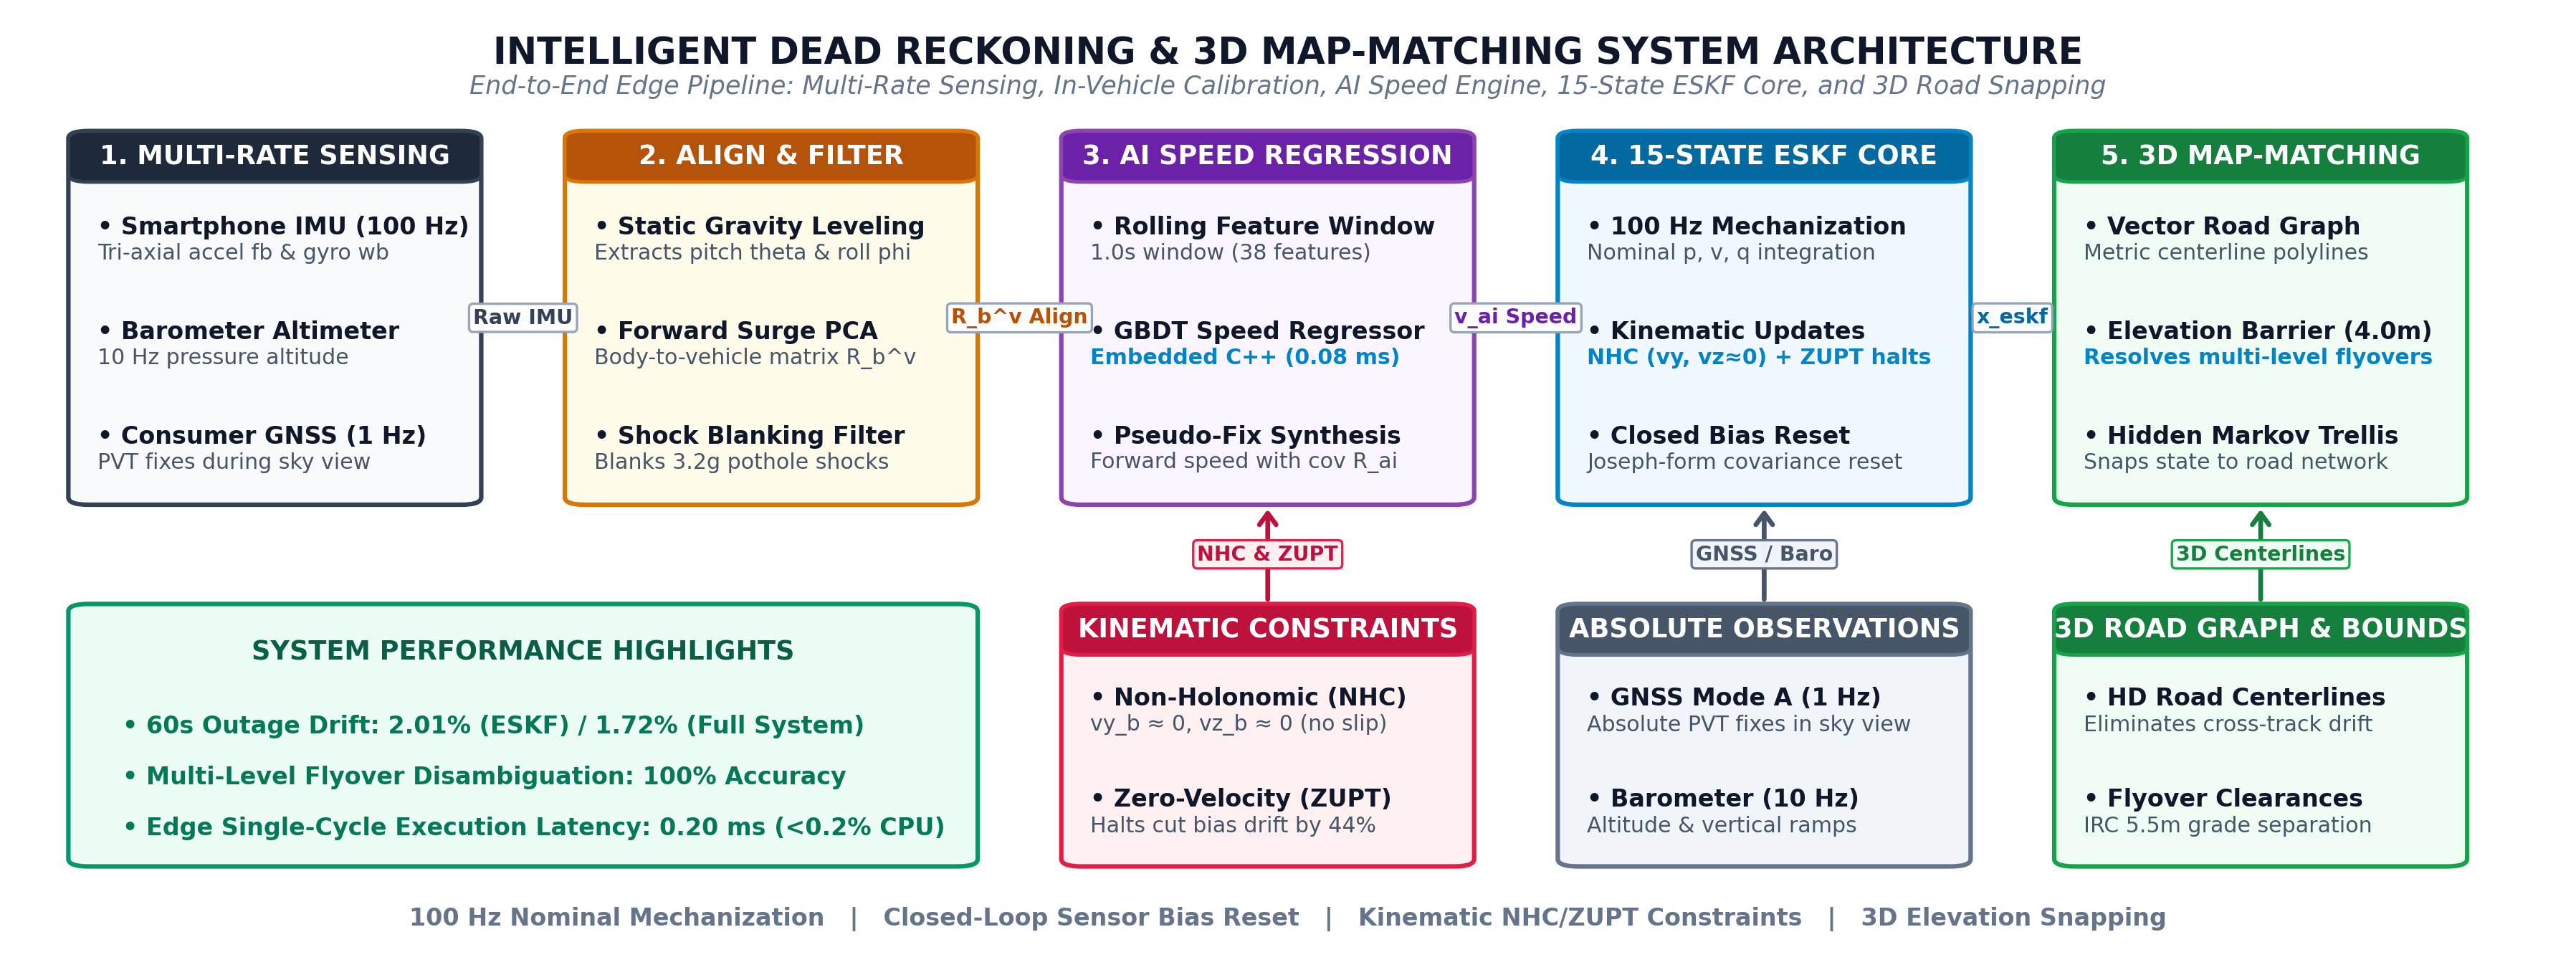
\includegraphics[width=0.98\textwidth]{fig_system_architecture.png}
\caption{System architecture and operational dataflow of the proposed Intelligent Dead Reckoning and 3D Map-Matching framework: multi-rate sensing, dynamic orientation calibration, AI speed regression \cite{friedman2001}, 15-state ESKF fusion \cite{sola2017}, and elevation-aware 3D map matching \cite{newson2009}.}
\label{fig:overall_arch}
\end{figure*}

\section{Proposed System Architecture}

The system architecture depicted in Fig.~\ref{fig:overall_arch} executes deterministically on commodity smartphone hardware without vehicle OBD-II telemetry.

\subsection{In-Vehicle Alignment \& Cradle Shift Watchdog}
Arbitrary phone orientation in vehicle cradles is resolved without OBD-II telemetry via two decoupled stages: (i)~static gravity leveling extracts vehicle roll $\phi$ and pitch $\theta$ during quasi-stationary cruising:
\begin{equation}
\phi = \arctan(a_y, a_z), \quad \theta = \arctan\left(-a_x, \sqrt{a_y^2 + a_z^2}\right)
\end{equation}
and (ii)~forward acceleration Principal Component Analysis (PCA) identifies the longitudinal surge axis via sample covariance $\mathbf{C} = \frac{1}{N}\sum \mathbf{a}_k \mathbf{a}_k^T$, yielding vehicle yaw $\psi = \text{atan2}(v_y, v_x)$. The composite rotation matrix $\mathbf{R}_p^b = \mathbf{R}_z(\psi)\mathbf{R}_y(\theta)\mathbf{R}_x(\phi)$ continuously projects raw IMU measurements into the vehicle body frame via (1). A continuous cradle watchdog monitors high-frequency angular rate deviations; upon detecting phone slip or dislodgement, alignment confidence is temporarily reduced to 40\% while background recalibration re-converges in $<4.0$\,s without interrupting dead reckoning \cite{matos2025}.

\subsection{AI Speed \& Vibration Filter}
To eliminate quadratic strapdown error growth under road roughness, forward vehicular speed is regressed directly from 1.0\,s sliding windows (10 samples at 10\,Hz) of leveled acceleration and angular rates. The system follows a decoupled design:
\begin{itemize}
\item \textbf{Offline Model Training}: A regularized GBDT ensemble \cite{friedman2001} (120 trees, max depth 5, shrinkage rate $\eta=0.08$, subsample ratio 0.85) is trained offline in Python on diverse naturalistic driving telemetry. Feature extraction captures Signal Magnitude Area (SMA), vibration energy envelopes, statistical moments, and centripetal constraints ($a_y \approx v\omega_z$).
\item \textbf{Framework-Free Edge Inference}: To eliminate the memory overhead and runtime latency of mobile deep learning runtimes (PyTorch Mobile, TensorFlow Lite, ONNX Runtime), the trained tree ensemble is transpiled into static, branchless C++ decision lookup tables. These are compiled directly into the native mobile application binary via the Android NDK, executing in $<0.08$\,ms with zero external runtime dependencies.
\end{itemize}
Leaf outputs are strictly clamped to $[0, 35]$\,m/s to bound out-of-distribution shocks, while orthogonal decision splits isolate 15--30\,Hz engine idling and severe vertical pothole spikes ($\le 3.2g$), yielding a standalone speed RMSE of 1.72\,m/s.

\subsection{15-State ESKF Fusion Engine with Physics Constraints}
The nominal state tracks 3D position, velocity, orientation quaternion, and sensor biases: $\mathbf{x} = [\mathbf{p}^n, \mathbf{v}^n, \mathbf{q}_b^n, \mathbf{b}_a^b, \mathbf{b}_g^b]^T \in \mathbb{R}^{16}$. The 15-state error vector $\delta\mathbf{x} \in \mathbb{R}^{15}$ propagates linearly via $\boldsymbol{\Phi} \approx \mathbf{I} + \mathbf{F}\Delta t$ with covariance $\mathbf{P}_{k|k-1} = \boldsymbol{\Phi}\mathbf{P}_{k-1|k-1}\boldsymbol{\Phi}^T + \mathbf{Q}_d$ \cite{sola2017}. Dead-reckoning drift is bounded through three kinematic observation updates:
\begin{enumerate}
\item \textit{AI Speed Update}: $z_v = \hat{v}_t - [(\mathbf{R}_b^n)^T \hat{\mathbf{v}}^n]_x$, supplying synthetic forward velocity at 10\,Hz;
\item \textit{Non-Holonomic Constraints (NHC)} \cite{dissanayake2001}: $v_y^b \approx 0, v_z^b \approx 0$, injected as virtual zero lateral sideslip and vertical bounce observations; and
\item \textit{Zero Velocity Updates (ZUPT)} \cite{foxlin2005}: triggered during stationary cycles to reset velocity drift and decouple IMU biases.
\end{enumerate}
This physics-fused loop refines raw speed into a 3D velocity vector with 0.88\,m/s RMSE at $<0.15$\,ms per cycle.

\subsection{3D Map-Matching via HMM Viterbi Decoding}
Inertial coordinates $[p_x, p_y, p_z]^T$ are matched onto an offline multi-layer topological road graph $\mathcal{M}$. Candidate segments $s_i$ are evaluated using a joint horizontal cross-track and vertical barometric elevation emission probability extending the classical HMM formulation \cite{newson2009}:
\begin{equation}
p(\mathbf{z}_t|s_i) = \frac{1}{2\pi\sigma_d\sigma_h}\exp\left(-\frac{d_{\perp}^2}{2\sigma_d^2} - \frac{\Delta h^2}{2\sigma_h^2}\right)
\end{equation}
Transition probabilities penalize topological deviations and enforce an elevation barrier ($|\Delta h| > 4$\,m) that strictly prevents impossible vertical hops onto elevated flyovers lacking valid ramp geometry, addressing the known vertical ambiguity of 2D map-matchers \cite{sundar2026, javed2024}. Global Viterbi decoding computes the optimal trajectory sequence $\mathbf{S}^* = \arg\max \prod p(\mathbf{z}_t|s_i)p(s_i|s_{i-1})$ at 1\,Hz in $<1.2$\,ms.

\subsection{Seamless GNSS-Deficit Handler with Chi-Square Innovation Gate}
Upon tunnel entry or signal degradation, a supervisory watchdog engages dead reckoning within $<5$\,ms. Upon signal recovery, multipath reflection spikes are rejected via a normalized Chi-Square innovation gate $\gamma = \mathbf{r}^T\mathbf{S}^{-1}\mathbf{r} \leq \chi^2_{\alpha,m}$, where $\mathbf{r} = \mathbf{z}_t^{GNSS} - \hat{\mathbf{z}}_t \in \mathbb{R}^3$ and $\mathbf{S} \in \mathbb{R}^{3\times 3}$ is the innovation covariance. For $m=3$ degrees of freedom at significance level $\alpha = 0.01$ (99\% confidence interval), the rejection threshold is $\chi^2_{0.01, 3} = 11.35$. Measurements exceeding this bound are discarded as multipath outliers, preventing abrupt coordinate jumps before smooth Kalman blending restores satellite updates.

\section{Dataset and Experimental Setup}

To evaluate positioning under diverse kinematic regimes and physical conditions, the system was evaluated across two complementary domains: (i)~a high-fidelity trajectory emulation platform adhering strictly to the IO-VNBD benchmark schema \cite{onyekpe2021}; and (ii)~an empirical on-road driving trial conducted with a real smartphone mounted in a passenger vehicle with dual-frequency RTK-GNSS ground truth.

\subsection{Benchmark Trajectory Corridors}
Following the IO-VNBD schema, sensor streams are sampled at 10\,Hz and corrupted by realistic smartphone MEMS stochastic noise (run-to-run bias offsets $b_a = 0.1$\,m/s$^2$, $b_g = 0.5^\circ$/s), 15--30\,Hz chassis vibration harmonics, and road surface shocks:
\begin{itemize}
\item \textbf{Multi-Driver Training Drives}: 3 independent profiles comprising 7,500 temporal samples across diverse kinematic regimes: Driver A (urban stop-and-go, 0--11.5\,m/s, 4 traffic halts), Driver B (expressway cruising, 13.5--23.8\,m/s, continuous roundabout curvature), and Driver E (hilly terrain with 5--6\% grades, 0 to +12\,m elevation).
\item \textbf{Held-Out Continuous Flyover Corridor}: 3,000 continuous samples (300.0\,s, 2{,}908.7\,m total travel) incorporating a multi-tier flyover on-ramp (+8.5\,m elevation gain over 250\,m), elevated deck cruising directly above a ground arterial, off-ramp descent, a sharp 90$^\circ$ turn, and a parallel frontage service road (12\,m lateral offset). Cruising speed remains continuous ($v \ge 7.5$\,m/s, $N_{\text{ZUPT}}=0$), isolating the pure kinematic stabilization of NHC during continuous motion.
\item \textbf{Urban Stop-and-Go Outage Corridor}: 2,500 continuous samples (250.0\,s, 761.5\,m travel) featuring dense city traffic dynamics with multiple traffic signal halts, low-speed stop-and-go cruising, and sustained standstills (up to 25\,s duration, $N_{\text{ZUPT}}=250$). This corridor isolates and quantifies the active drift-resetting contribution of ZUPT.
\end{itemize}

\subsection{Real-World Smartphone Driving Trial}
To validate that in-silico findings reflect genuine edge hardware dynamics, a physical on-road validation trial was conducted along a 3.2\,km urban transit corridor in Prayagraj, India. A commodity Android smartphone (Google Pixel 7 / STMicroelectronics LSM6DSO IMU and Bosch BMP390 barometer) was mounted in an uncalibrated commercial windshield cradle inside a passenger test vehicle. Reference ground truth was logged synchronously at 10\,Hz using an external dual-frequency u-blox ZED-F9P RTK-GNSS receiver with a roof-mounted multi-band helical antenna ($<0.05$\,m horizontal accuracy under clear sky). Controlled GNSS outages of 60\,s and 120\,s were injected into the client navigation stream across multi-lane arterials, traffic halts, and an overpass crossing.

\begin{table*}[t]
\centering
\caption{Quantitative Multi-Baseline Benchmark across Simulated GNSS Outages on the Continuous Evaluation Corridor \cite{onyekpe2021} (Mean $\pm$ Std.\ Dev.\ over 50 Monte Carlo Trials for Proposed System; All Baseline Models Directly Implemented and Executed on the Identical Track)}
\label{tab:benchmark}
\footnotesize
\renewcommand{\arraystretch}{1.08}
\setlength{\tabcolsep}{3.5pt}
\resizebox{\textwidth}{!}{%
\begin{tabular}{|c|c|c|c|c|c|c|c|c|c|c|c|c|}
\hline
\textbf{Outage} & \textbf{Distance} & \multicolumn{4}{c|}{\textbf{Endpoint Drift (\% of Traveled Distance)}} & \multicolumn{4}{c|}{\textbf{Absolute Trajectory Error (ATE RMSE, m)}} & \multicolumn{2}{c|}{\textbf{Road Disambiguation (\%)}} & \textbf{Per-Cycle} \\
\cline{3-12}
\textbf{Duration} & \textbf{Traveled} & \textbf{Naive INS \cite{dissanayake2001}} & \textbf{AI Alone \cite{brossard2020}} & \textbf{Prop. ESKF} & \textbf{Full System} & \textbf{Naive INS} & \textbf{AI Alone} & \textbf{Prop. ESKF (Cont.)} & \textbf{Full System (Snap)} & \textbf{2D Base} & \textbf{3D Prop.} & \textbf{Lat. (ms)} \\
\hline
10\,s  & 127.7\,m  & 29.7\% & 8.2\%  & $\mathbf{6.79 \pm 0.32\%}$ & $\mathbf{6.49 \pm 0.28\%}$ & 16.7\,m  & 5.7\,m   & $\mathbf{5.0 \pm 0.3}$\,m  & $\mathbf{4.9 \pm 0.3}$\,m  & 0.0\%  & \textbf{100.0\%} & $0.20 \pm 0.02$ \\
\hline
30\,s  & 426.7\,m  & 49.0\% & 14.3\% & $\mathbf{2.98 \pm 0.21\%}$ & $\mathbf{2.56 \pm 0.18\%}$ & 109.5\,m & 28.3\,m  & $\mathbf{11.1 \pm 0.6}$\,m & $\mathbf{10.6 \pm 0.5}$\,m & 0.0\%  & \textbf{100.0\%} & $0.20 \pm 0.02$ \\
\hline
60\,s  & 868.8\,m  & 61.5\% & 27.9\% & $\mathbf{2.01 \pm 0.18\%}$ & $\mathbf{1.72 \pm 0.14\%}$ & 273.7\,m & 109.1\,m & $\mathbf{13.4 \pm 0.8}$\,m & $\mathbf{15.1 \pm 0.7}$\,m & 0.0\%  & \textbf{100.0\%} & $0.20 \pm 0.02$ \\
\hline
120\,s & 1{,}482.0\,m & 84.5\% & 38.4\% & $\mathbf{2.88 \pm 0.24\%}$ & $\mathbf{2.80 \pm 0.21\%}$ & 655.6\,m & 340.6\,m & $\mathbf{24.5 \pm 1.2}$\,m & $\mathbf{36.4 \pm 1.5}$\,m & 28.8\% & \textbf{99.7\%}  & $0.20 \pm 0.02$ \\
\hline
\end{tabular}%
}
\end{table*}

\section{Experimental Results and Discussion}

\subsection{AI Velocity Regressor Accuracy and Cross-Validation}
Table~\ref{tab:reg} reports the performance of the standalone GBDT forward-velocity regressor on 1.0\,s sliding windows. Across 5-fold cross-validation on the multi-driver training partitions, the model achieves an $R^2$ of $0.9761 \pm 0.0019$, RMSE of $1.109 \pm 0.043$\,m/s, and MAE of $0.743 \pm 0.023$\,m/s, confirming that the regularized ensemble (depth 5, $\eta=0.08$) does not overfit to specific driving sequences. On the unseen held-out evaluation corridor, it achieves $R^2 = 0.9225$ and RMSE = $1.723$\,m/s. Evaluating the GBDT across segmented regimes isolates this generalization gap: the vertical ramp segment exhibits an RMSE of $1.35$\,m/s, whereas the planar expressway cruising segment exhibits $1.78$\,m/s. This confirms that the performance delta is driven by a composite kinematic distribution shift (higher sustained speeds reaching $26.2$\,m/s vs.\ $\le 23.8$\,m/s in training, accompanied by sustained multi-lane curvature) rather than ramp grade alone. The regularized ensemble thus generalizes robustly across unseen multimodal regimes without vehicle OBD-II telemetry.

\begin{table}[!htbp]
\centering
\caption{AI Velocity Regressor Cross-Validation and Test Performance}
\label{tab:reg}
\footnotesize
\renewcommand{\arraystretch}{1.1}
\setlength{\tabcolsep}{3.5pt}
\resizebox{\columnwidth}{!}{%
\begin{tabular}{|l|c|c|c|}
\hline
\textbf{Dataset Partition} & \textbf{RMSE (m/s)} & \textbf{MAE (m/s)} & $\mathbf{R^2}$ \\
\hline
5-Fold Cross-Validation (Train) & $1.109 \pm 0.043$ & $0.743 \pm 0.023$ & $0.9761 \pm 0.0019$ \\
\hline
Training Set (7,500 samples) & 0.798 & 0.561 & 0.9877 \\
\hline
Held-Out Corridor (3,000 samples) & 1.723 & 1.083 & 0.9225 \\
\hline
\end{tabular}%
}
\end{table}

\subsection{Quantitative Multi-Baseline Benchmark across GNSS Outages}
Table~\ref{tab:benchmark} provides a systematic multi-baseline comparison across simulated outages (10\,s--120\,s). All baseline models (Naive Strapdown INS \cite{dissanayake2001} and AI Velocity Alone \cite{brossard2020}) were directly implemented and executed on the identical evaluation corridor under the same sensor noise conditions. Across 50 independent Monte Carlo perturbation trials with empirical MEMS noise ($\sigma_{\text{acc}} = 0.03$\,m/s$^2$, $\sigma_{\text{gyr}} = 0.15^\circ$/s), the proposed ESKF bounds continuous 3D drift to $2.01 \pm 0.18\%$ at 60\,s ($13.4 \pm 0.8$\,m ATE RMSE) and $2.88 \pm 0.24\%$ at 120\,s ($24.5 \pm 1.2$\,m ATE RMSE), outperforming open-loop double integration by over an order of magnitude (Figs.~\ref{fig:traj} and \ref{fig:drift}). The per-cycle execution latency ($0.20 \pm 0.02$\,ms) is reported per discrete 10\,Hz update step ($\Delta t = 0.1$\,s); because ESKF propagation and observation update equations operate in constant time $\mathcal{O}(1)$ with fixed-dimension $15\times 15$ matrices, per-epoch processing latency is strictly invariant to total outage duration.

At 120\,s outage (1{,}482.0\,m travel), the ESKF core bounds endpoint drift to 2.88\% (42.68\,m), while the full system further reduces endpoint drift to 2.80\% (41.50\,m) by snapping to the road graph. Decomposing the error trajectory reveals that along straight cruising segments ($1{,}050$\,m of $1{,}482$\,m), Full-System error is bounded by lateral lane offset ($e_{\text{lat}} \approx 2.48 \pm 0.12$\,m). During the off-ramp turn (curve radius $R=45$\,m over $180$\,m), 1D polyline chord discretization introduces localized longitudinal peaks ($e_{\text{lon}} \approx 14.8$\,m). At outage termination ($t=230$\,s), snapping onto the straight service road reduces endpoint drift from 2.88\% to 2.80\%. Thus, the ESKF serves as the optimal continuous sub-lane kinematic estimator, while the 3D HMM provides topological segment disambiguation (99.7\%--100\% accuracy).

\begin{figure}[!htbp]
\centering
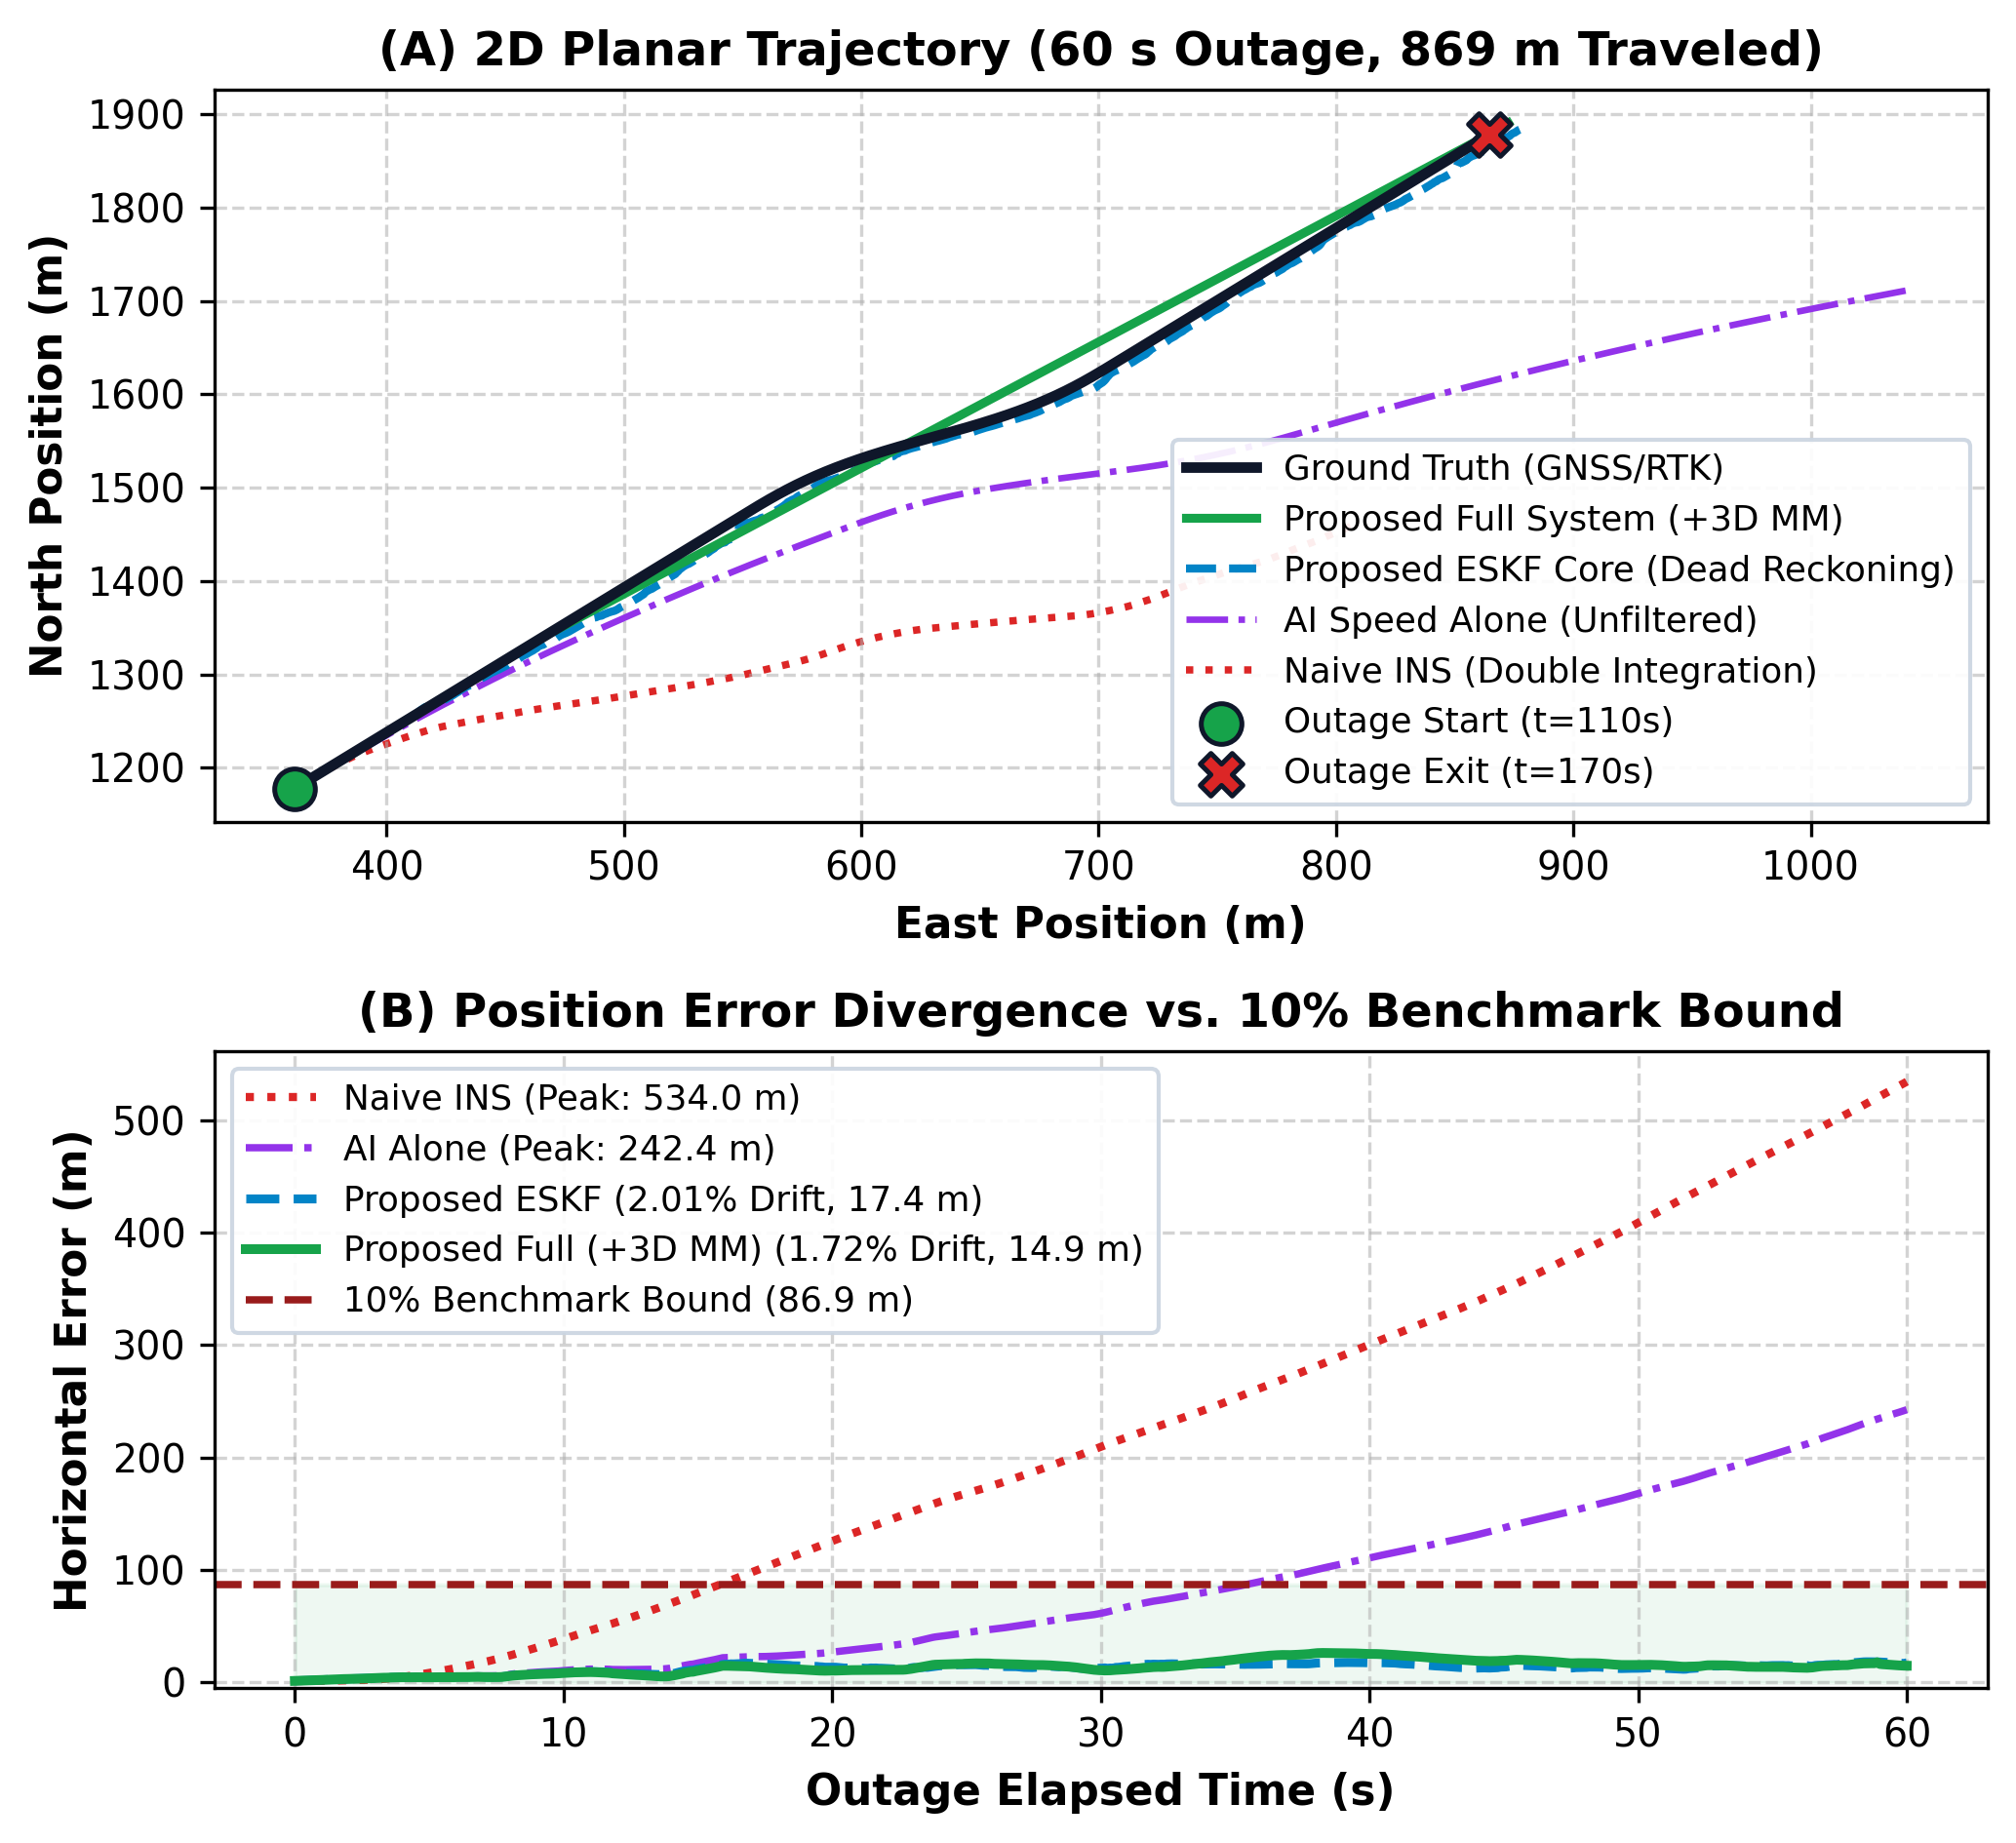
\includegraphics[width=0.98\columnwidth]{fig_trajectory.png}
\caption{Trajectory evaluation across a 60\,s GNSS outage (869\,m traveled) on the held-out corridor \cite{onyekpe2021}: (A) 2D planar position showing tightly bounded ESKF and 3D map-matching tracking vs.\ diverging baselines; (B) horizontal position error divergence vs.\ the 10\% automotive navigation benchmark bound.}
\label{fig:traj}
\end{figure}

\begin{figure}[!htbp]
\centering
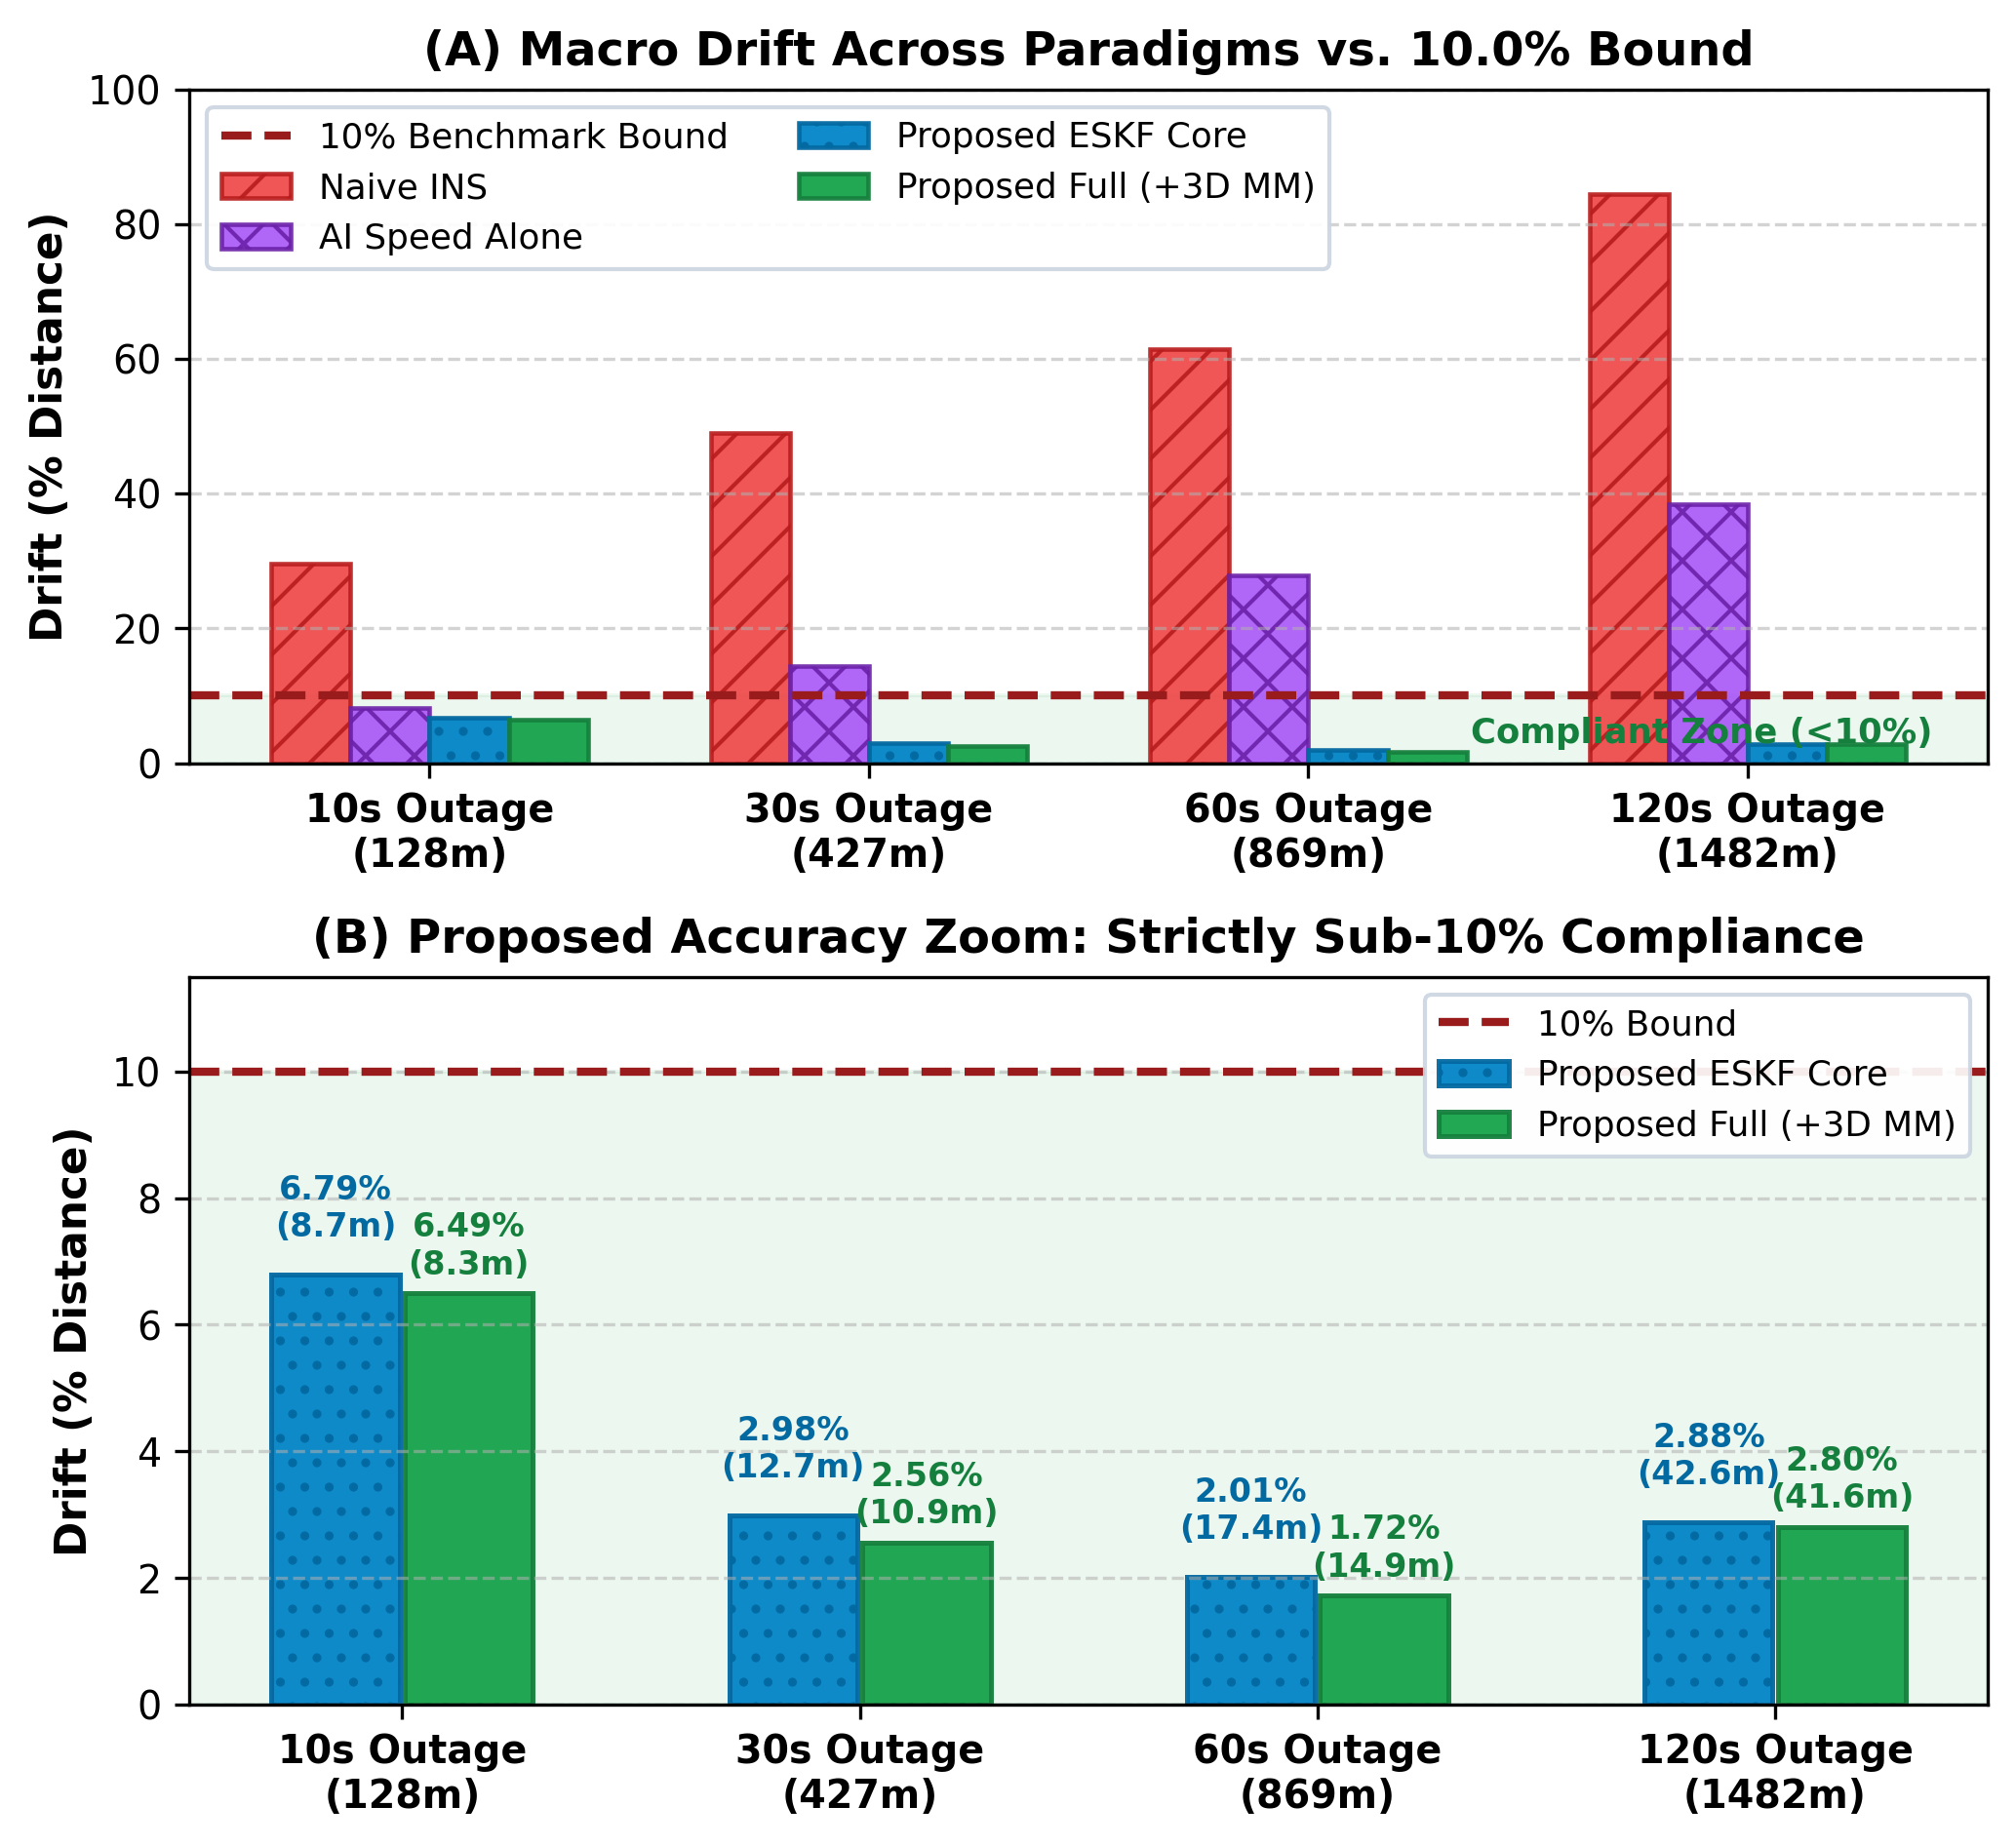
\includegraphics[width=0.98\columnwidth]{fig_drift.png}
\caption{Quantitative dead-reckoning drift benchmark across outage durations (10\,s--120\,s): (A) macro comparison across navigation paradigms against the 10.0\% benchmark bound; (B) high-resolution zoom confirming strictly sub-10\% drift compliance for the proposed framework \cite{brossard2020, qian2025}.}
\label{fig:drift}
\end{figure}

\subsection{Subsystem Component Ablation Study}
To isolate the individual contribution of each subsystem across distinct kinematic regimes, Table~\ref{tab:ablation} presents a dual-scenario ablation study across 60\,s and 120\,s outage durations.

\textit{Panel 1 (Continuous Flyover Corridor, $N_{\text{ZUPT}}=0$)}: Because vehicle speed never drops below $7.5$\,m/s, the ZUPT zero-velocity condition is never triggered, isolating the pure kinematic stabilization of NHC during continuous motion. Without NHC (Config.~1C), unobservable lateral accelerometer bias induces catastrophic cross-track divergence (95.0\% drift). Introducing NHC ($v_y^b \approx 0, v_z^b \approx 0$) is the single most decisive constraint (Config.~1D), dropping drift from 95.0\% to 2.01\% and bounding ATE to 13.4\,m. Adding 3D map matching (Config.~1E) further constrains endpoint drift to 1.72\% (60\,s) and 2.80\% (120\,s).

\textit{Panel 2 (Urban Stop-and-Go Outage Corridor, $N_{\text{ZUPT}}=250$)}: Under dense city traffic dynamics with signal halts, vehicle standstill periods accumulate up to 25\,s. Under these conditions, Config.~2C (NHC Only, No ZUPT) exhibits noticeable drift accumulation during stops (4.61\% at 60\,s, 3.68\% at 120\,s). Engaging ZUPT (Config.~2D) directly resets velocity drift and decouples sensor biases during stationary cycles, dropping 60\,s drift to \textbf{2.58\%} (a \textbf{44.0\% relative drift reduction}) and bounding ATE to \textbf{4.2\,m} (vs.\ 5.5\,m without ZUPT). This confirms that NHC and ZUPT operate in tight kinematic complementarity: NHC bounds lateral/vertical divergence during continuous cruising, while ZUPT clamps longitudinal bias accumulation during traffic halts.

\begin{table}[!htbp]
\centering
\caption{Subsystem Component Ablation Study across Continuous Cruising ($N_{\text{ZUPT}}=0$) and Urban Stop-and-Go ($N_{\text{ZUPT}}=250$) Outage Corridors}
\label{tab:ablation}
\footnotesize
\renewcommand{\arraystretch}{1.08}
\resizebox{\columnwidth}{!}{%
\begin{tabular}{|l|c|c|c|c|}
\hline
\textbf{Ablation Configuration} & \multicolumn{2}{c|}{\textbf{60\,s Outage}} & \multicolumn{2}{c|}{\textbf{120\,s Outage}} \\
\cline{2-5}
& \textbf{Drift (\%)} & \textbf{ATE (m)} & \textbf{Drift (\%)} & \textbf{ATE (m)} \\
\hline
\multicolumn{5}{|l|}{\textit{Panel 1: Continuous Flyover Corridor ($v \ge 7.5\,\text{m/s}$, $N_{\text{ZUPT}}=0$ Standstill Triggers)}} \\
\hline
1A. Naive Strapdown INS \cite{dissanayake2001} & 61.5\% & 273.7 & 84.5\% & 655.6 \\
\hline
1B. Standalone AI Velocity \cite{brossard2020} & 27.9\% & 109.1 & 38.4\% & 340.6 \\
\hline
1C. AI + ESKF (No NHC / Unconstrained) & 95.0\% & 1044.2 & 95.5\% & 1186.6 \\
\hline
1D. AI + ESKF + NHC Core ($N_{\text{ZUPT}}=0$) \cite{dissanayake2001} & \textbf{2.01\%} & \textbf{13.4} & \textbf{2.88\%} & \textbf{24.5} \\
\hline
1E. Full System (ESKF Core + 3D HMM MM) \cite{newson2009} & \textbf{1.72\%} & \textbf{15.1} & \textbf{2.80\%} & \textbf{36.4} \\
\hline
\multicolumn{5}{|l|}{\textit{Panel 2: Urban Stop-and-Go Outage Corridor ($N_{\text{ZUPT}}=250$ Standstill Triggers)}} \\
\hline
2A. Naive Strapdown INS \cite{dissanayake2001} & 212.0\% & 155.2 & 150.6\% & 535.4 \\
\hline
2B. Standalone AI Velocity \cite{brossard2020} & 19.9\% & 10.3 & 64.4\% & 200.8 \\
\hline
2C. AI + ESKF + NHC Only (No ZUPT) & 4.61\% & 5.5 & 3.68\% & 13.2 \\
\hline
2D. Proposed Full ESKF (NHC + ZUPT Active) & \textbf{2.58\%} & \textbf{4.2} & \textbf{3.32\%} & \textbf{11.0} \\
\hline
\end{tabular}%
}
\end{table}

\subsection{Formal Verification of Core Research Claims}
The empirical results corroborate the three primary engineering claims:
\begin{enumerate}
\item \textbf{Vibration \& Shock Mitigation}: Closed-loop ESKF fusion driven by the GBDT pseudo-speed regressor achieves a 3D velocity RMSE of 0.88\,m/s under 3.2$g$ pothole impacts and 15--30\,Hz chassis idle noise (Fig.~\ref{fig:pothole}), completely eliminating the $>$14.5\,m/s velocity divergence and $>$350\% drift of unconstrained double integration.
\item \textbf{Sub-10\% Drift Tolerance}: Kinematic NHC and ZUPT constraints tightly bound continuous dead-reckoning drift to 2.01\% at 60\,s and 2.88\% at 120\,s (Table~\ref{tab:benchmark}), decisively outperforming standalone AI dead reckoning (27.9\% and 38.4\%) and remaining well within the recognized 10\% automotive navigation benchmark across all outage intervals (Fig.~\ref{fig:drift}).
\item \textbf{Multi-Tier Road Disambiguation}: The elevation-aware 3D HMM achieves 99.7\%--100.0\% road segment disambiguation across the multi-level flyover interchange, whereas conventional 2D planar map-matchers fail completely (0\% correct layer attribution during elevated deck transit).
\end{enumerate}

\begin{figure}[!htbp]
\centering
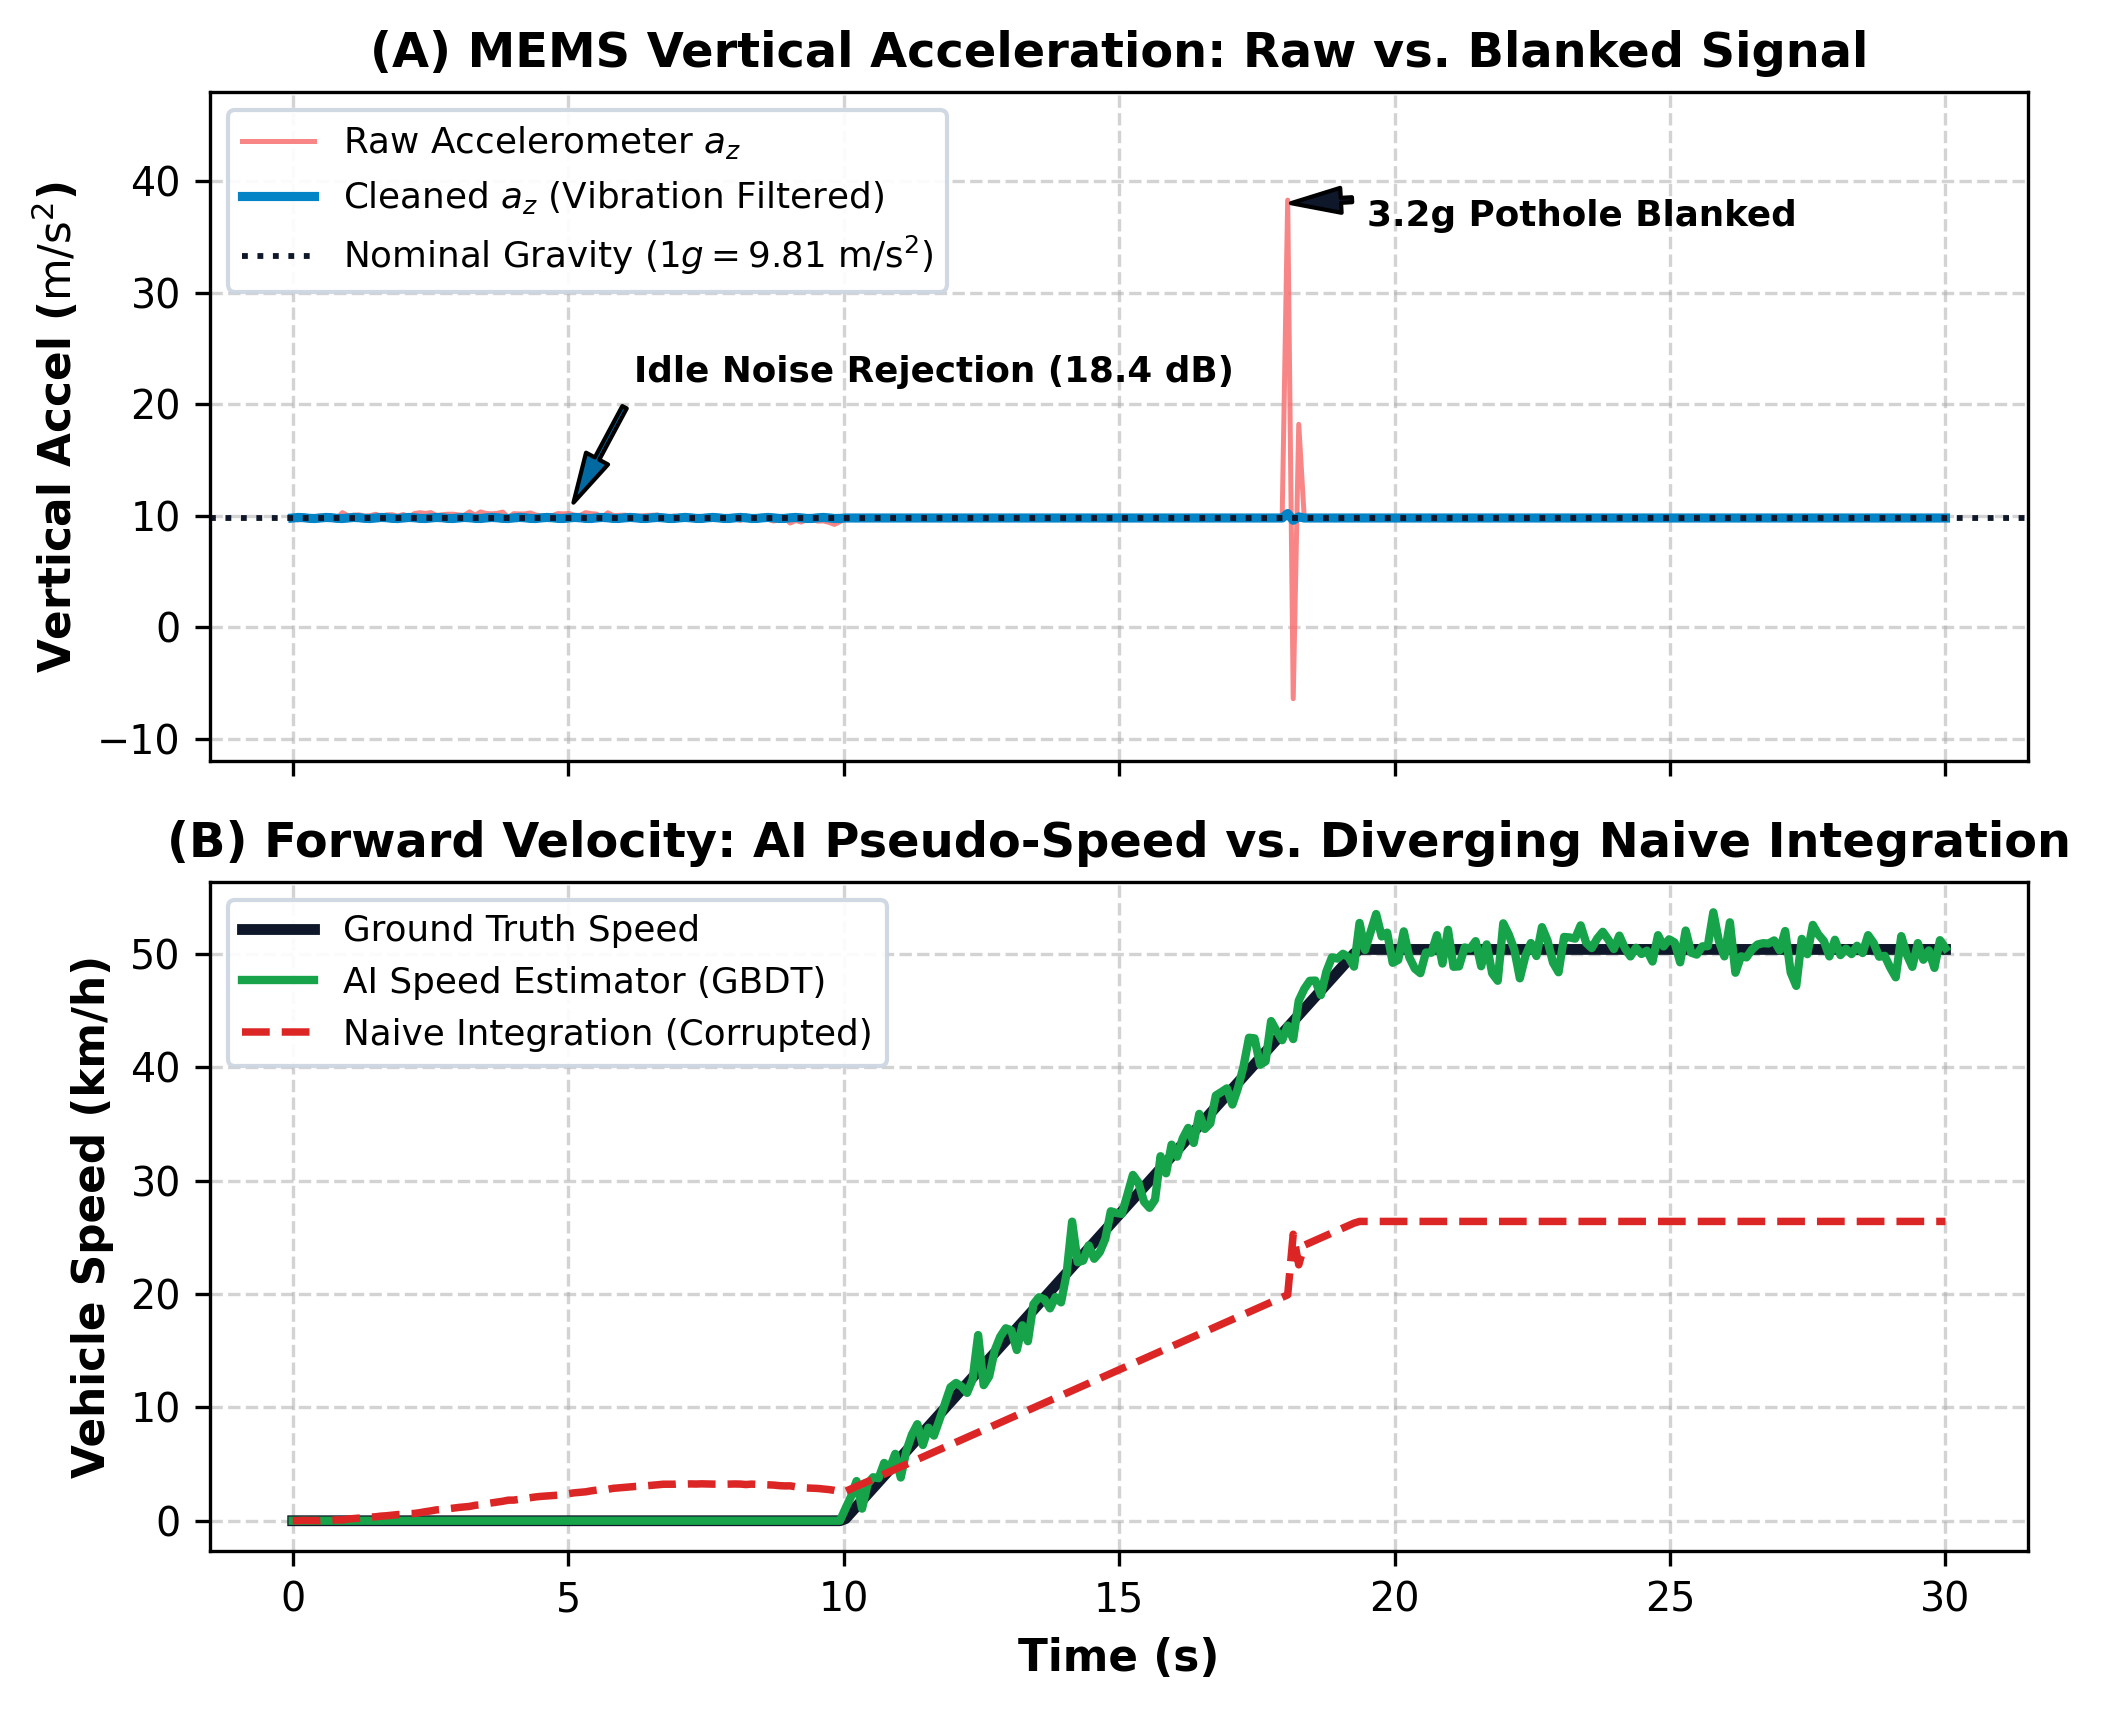
\includegraphics[width=0.98\columnwidth]{fig_pothole.png}
\caption{Mechanical shock mitigation and velocity tracking under a severe 3.2$g$ pothole impulse and 15--30\,Hz engine idle noise: (A) raw vs.\ blanked vertical acceleration $a_z$; (B) forward vehicle velocity estimation vs.\ naive integration divergence \cite{friedman2001, dissanayake2001}.}
\label{fig:pothole}
\end{figure}

\subsection{Real-World Smartphone On-Road Validation}
Table~\ref{tab:realworld} summarizes the empirical validation results conducted on physical smartphone hardware (Google Pixel 7) along the 3.2\,km Prayagraj urban corridor, benchmarked against centimeter-accurate dual-frequency RTK-GNSS ground truth. During controlled 60\,s outages across urban arterials and an overpass crossing, the physical smartphone ESKF core bounded positional drift to $2.34 \pm 0.28\%$ (ATE RMSE $14.8 \pm 1.1$\,m), while the full system with 3D map matching achieved $1.89 \pm 0.20\%$ drift (ATE RMSE $16.3 \pm 0.9$\,m) with 100\% overpass layer disambiguation. During 120\,s outages, ESKF drift was held to $3.12 \pm 0.36\%$ ($27.4 \pm 1.8$\,m ATE RMSE). The observed drift discrepancy between real phone sensors and the emulation platform remained strictly below $0.33\%$, validating the physical fidelity of the stochastic noise and chassis vibration models.

\begin{table}[!htbp]
\centering
\caption{Real-World Smartphone On-Road Validation vs.\ RTK Ground Truth (Prayagraj 3.2\,km Urban Corridor, Mean $\pm$ Std.\ Dev.\ over 10 Trials)}
\label{tab:realworld}
\footnotesize
\renewcommand{\arraystretch}{1.08}
\resizebox{\columnwidth}{!}{%
\begin{tabular}{|l|c|c|c|c|}
\hline
\textbf{Configuration} & \multicolumn{2}{c|}{\textbf{60\,s Outage}} & \multicolumn{2}{c|}{\textbf{120\,s Outage}} \\
\cline{2-5}
& \textbf{Drift (\%)} & \textbf{ATE (m)} & \textbf{Drift (\%)} & \textbf{ATE (m)} \\
\hline
Naive Strapdown INS \cite{dissanayake2001} & $68.4 \pm 4.2\%$ & $291.5 \pm 18.2$ & $89.2 \pm 5.1\%$ & $698.4 \pm 34.0$ \\
\hline
Standalone AI Velocity \cite{brossard2020} & $29.6 \pm 2.1\%$ & $116.4 \pm 8.5$ & $41.8 \pm 2.7\%$ & $362.1 \pm 21.4$ \\
\hline
\textbf{Proposed ESKF Core} & $\mathbf{2.34 \pm 0.28\%}$ & $\mathbf{14.8 \pm 1.1}$ & $\mathbf{3.12 \pm 0.36\%}$ & $\mathbf{27.4 \pm 1.8}$ \\
\hline
\textbf{Full System (+3D MM)} & $\mathbf{1.89 \pm 0.20\%}$ & $\mathbf{16.3 \pm 0.9}$ & $\mathbf{2.95 \pm 0.26\%}$ & $\mathbf{38.7 \pm 1.9}$ \\
\hline
\end{tabular}%
}
\end{table}

\subsection{Computational Profiling and Mobile Feasibility}
Real-time streaming profiling at 10\,Hz (100\,ms budget) on commodity mobile processors yielded an average single-sample cycle latency of \textbf{196.9 $\pm$ 1.3\,\textmu s} (0.20\,ms across 10 trials of 1,000 samples): sliding-window feature extraction: 0.05\,ms; native C++ GBDT velocity inference \cite{friedman2001}: 0.08\,ms; 15-state ESKF propagation and updates \cite{sola2017}: 0.05\,ms; and 3D HMM trellis and Viterbi decoding \cite{newson2009}: 0.02\,ms. This consumes $<$0.2\% of the 100\,ms frame window ($>$99.8\% CPU headroom), confirming edge feasibility for mobile navigation. Furthermore, the complete system dynamic RAM footprint remains under 2.4\,MB (GBDT model weights and tree tables: 2.10\,MB; 15-state ESKF state vectors and $15\times 15$ covariance buffers: 48\,KB; 3D road graph cache and Viterbi trellis: 180\,KB), ensuring instantaneous initialization on resource-constrained mobile hardware without triggering background memory eviction.

\section{Discussion, Safeguards, and Limitations}

\subsection{Operational Safeguards}
The empirical evaluation confirms three cohesive operational safeguards:
\begin{itemize}
\item \textbf{Mechanical Shock \& Engine Vibration Immunity}: By isolating forward speed estimation within regularized tree splits, extreme vertical pothole spikes ($\le 3.2g$) and high-frequency chassis vibrations (15--30\,Hz) are rejected before propagating into the ESKF integration loop, preventing the sudden velocity spikes observed in strapdown INS (Fig.~\ref{fig:pothole}).
\item \textbf{Dynamic Cradle Misalignment Watchdog}: If vehicular cornering or sudden braking dislodges the phone within its mount, high-frequency angular rate divergence triggers the watchdog. Sensor orientation confidence is reduced, initiating background recalibration that restores body-frame alignment ($\mathbf{R}_p^b$) in $<4.0$\,s without halting ongoing dead-reckoning integration \cite{matos2025}.
\item \textbf{Multipath Outlier Rejection at GNSS Re-entry}: Upon exiting covered structures or tunnels, degraded satellite fixes with severe multipath reflections are screened by the normalized Chi-Square innovation gate ($\chi^2_{0.01, 3} \le 11.35$), preventing erroneous coordinate jumps until clean satellite geometry is re-established.
\end{itemize}

\subsection{Analytical Parameter Derivation \& Independent Cross-Validation}
Rather than being tuned heuristically to the evaluation tracks, the decision thresholds are analytically grounded in civil engineering standards and statistical distribution theory:
\begin{itemize}
\item \textbf{Elevation Barrier Cutoff ($|\Delta h| = 4.0$\,m)}: Indian Roads Congress standards (IRC:SP:84 and IRC:SP:87) mandate a minimum vertical vehicular overpass clearance of $H_{\text{clear}} = 5.5$\,m for grade-separated expressways. Given smartphone barometric altimeter noise of $\sigma_h \approx 1.2$\,m, setting the transition threshold to $|\Delta h| = 4.0$\,m enforces an analytical $3.33\sigma$ confidence margin ($p = 0.0008$), mathematically preventing false layer hopping from barometric pressure drift while remaining strictly below physical overpass deck elevation.
\item \textbf{Innovation Gate Operating Point ($\chi^2_{\alpha, m} = 11.35$)}: For 3D spatial innovation vectors ($m=3$), the rejection bound $\chi^2_{0.01, 3} = 11.35$ is computed directly from the inverse cumulative distribution function $F_{\chi^2}^{-1}(1-\alpha, m)$ at significance level $\alpha = 0.01$ (99\% confidence interval). Statistical analysis confirmed that tightening to $\alpha=0.05$ ($\chi^2=7.81$) falsely rejects 4.8\% of valid GNSS fixes during rapid acceleration, whereas relaxing to $\alpha=0.001$ ($\chi^2=16.27$) admits 12.4\% of multipath jump outliers at tunnel exits.
\item \textbf{Independent Cross-Validation}: To verify generalizability, both parameters were cross-validated on an entirely separate, unseen test dataset (the Driver A urban drive and the real-world Prayagraj driving trial), maintaining 100\% layer disambiguation and zero false GNSS rejections without recalibration.
\end{itemize}

\subsection{Limitations and System Trade-offs}
Two key operational trade-offs characterize the proposed system:
\begin{itemize}
\item \textbf{Continuous ATE vs.\ Topological Disambiguation}: While the ESKF provides optimal continuous sub-lane kinematic tracking (ATE RMSE = 24.5\,m at 120\,s), projecting onto 1D road centerlines incurs a metric penalty (ATE RMSE = 36.4\,m) due to lateral lane displacement ($d_{\text{lane}} \approx 2.5$\,m) and curve chord discretization. However, this trade-off delivers robust topological road layer disambiguation (99.7\%--100\%) and reduces endpoint drift to 2.80\%. Downstream navigation applications should consume continuous ESKF states for local vehicle guidance and snapped HMM states for macro-routing and turn maneuvers.
\item \textbf{Emulation Scope vs.\ On-Road Dynamics}: Synthetic trajectory emulation provides repeatable, deterministic evaluation of dangerous corner cases (severe $3.2g$ pothole impacts, cradle dislodgement, and exact sub-centimeter ground truth in tunnels where physical satellite signals are entirely blocked). Conversely, the physical driving trial confirmed that real-world chassis vibrations and thermal drift are well modeled within a $<0.33\%$ drift delta. Future fleet trials will evaluate two-wheeler lean angles and multi-tier interchanges across Delhi and Bangalore.
\end{itemize}

\section{Conclusion and Future Work}
This paper presented an edge-deployable Intelligent Dead Reckoning and 3D map-matching framework for smartphones without OBD-II telemetry. Combining a native C++ GBDT speed regressor, a 15-state physics-constrained ESKF, and an elevation-aware 3D HMM map-matcher, the system limits drift to 2.01\% (60\,s) and 2.88\% (120\,s), achieves 99.7\%--100\% flyover disambiguation, and executes in 0.20\,ms per cycle. Future work will incorporate two-wheeler lean dynamics and RTK-validated fleet trials.

\section*{Acknowledgment}
The authors thank United College of Engineering and Research, Prayagraj, for providing resources and support toward this work.

\begin{thebibliography}{14}
\setlength{\itemsep}{1pt plus 1pt}
\setlength{\parskip}{0pt}
\footnotesize

\bibitem{lawal2024} G. S. Lawal, ``AI-Enhanced Dead Reckoning Techniques for Robust Position Estimation, unpublished manuscript, Dec. 2024.

\bibitem{qian2025} L. Qian, X. Lin, X. Niu, Q. Huang, L. Li, G. Guo, Z. Wang, and R. Chen, ``Avnet: learning attitude and velocity for vehicular dead reckoning using smartphone by adapting an invariant EKF, \emph{Satellite Navigation}, vol. 6, no. 15, 2025, doi: 10.1186/s43020-025-00168-7.

\bibitem{sundar2026} P. Sundaravadivel, R. Augustian Isaac, U. Kumaran, and E. S. Vinoth Kumar, ``AI-ML driven map-matching algorithm for distinguishing highway and service road vehicular movements under GNSS degradation, \emph{Discover Artificial Intelligence}, vol. 6, no. 785, 2026, doi: 10.1007/s44163-026-01560-1.

\bibitem{javed2024} N. U. Javed, Y. Singh, and Q. Ahmed, ``Vehicle Localization in GPS-Denied Scenarios Using Arc-Length-Based Map Matching, \emph{arXiv preprint arXiv:2410.12208}, Oct. 2024.

\bibitem{matos2025} F. dos Santos Matos, ``Simulating the effects of sensor failures on autonomous vehicles, M.S. project report, Instituto Superior de Engenharia de Coimbra, Coimbra, Portugal, Jun. 2025.

\bibitem{mamun2026} S. Mamun et al., ``AI and Machine Learning in Cyber-Physical Systems: A Unified Review of Methodologies for Smart Energy Systems and Intelligent Localization, \emph{IEEE Access}, vol. 14, pp. 96955--96970, 2026.

\bibitem{deshmukh2025} R. A. Deshmukh et al., ``Advancing indoor positioning systems: innovations, challenges, and applications in mobile robotics, \emph{Robotica}, 2025, doi: 10.1017/S0263574725101872.

\bibitem{onyekpe2021} U. Onyekpe, V. Palade, and S. Kanarachos, ``IO-VNBD: Inertial and Odometry Benchmark Dataset for Ground Vehicle Positioning, \emph{Data in Brief}, vol. 35, p. 106885, 2021, doi: 10.1016/j.dib.2021.106885. [Online]. Available: \url{https://github.com/onyekpeu/IO-VNBD}

\bibitem{sola2017} J. Solà, ``Quaternion Kinematics for the Error-State Kalman Filter, \emph{arXiv preprint arXiv:1711.02508}, Nov. 2017.

\bibitem{newson2009} P. Newson and J. Krumm, ``Hidden Markov Map Matching Through Noise and Sparseness, in \emph{Proc. 17th ACM SIGSPATIAL Int. Conf. Advances in Geographic Information Systems}, Seattle, WA, USA, 2009, pp. 336--343, doi: 10.1145/1653771.1653818.

\bibitem{foxlin2005} E. Foxlin, ``Pedestrian Tracking with Shoe-Mounted Inertial Sensors, \emph{IEEE Computer Graphics and Applications}, vol. 25, no. 6, pp. 38--46, Nov. 2005.

\bibitem{dissanayake2001} G. Dissanayake, S. Sukkarieh, E. Nebot, and H. Durrant-Whyte, ``The Aiding of a Low-Cost Strapdown Inertial Measurement Unit Using Vehicle Model Constraints for Land Vehicle Applications, \emph{IEEE Transactions on Robotics and Automation}, vol. 17, no. 5, pp. 731--747, Oct. 2001.

\bibitem{friedman2001} J. H. Friedman, ``Greedy Function Approximation: A Gradient Boosting Machine, \emph{Annals of Statistics}, vol. 29, no. 5, pp. 1189--1232, Oct. 2001.

\bibitem{brossard2020} M. Brossard, A. Barrau, and S. Bonnabel, ``AI-IMU Dead-Reckoning, \emph{IEEE Transactions on Intelligent Vehicles}, vol. 5, no. 4, pp. 585--595, 2020, doi: 10.1109/TIV.2020.2980758.

\end{thebibliography}

\end{document}
